\chapter{Series}
When writing a number with an infinite decimal, such as the Golden 
Ratio (also known as the Golden Number):
$$\phi = 1.618033988 \cdots$$

The decimal system means we can re-write the Golden Ratio (or any 
irrational number) as an infinite sum:
$$\phi = 1 + \frac{6}{10} + \frac{1}{10^2} + \frac{8}{10^3} + 
\frac{0}{10^4} + \frac{3}{10^5} + \cdots$$

You might recall from the chapter on Riemann Sums that we can 
represent the addition of many (or infinite) with big sigma notation:
$$\sum_{i = 1}^n a_i$$
Where i is the index as discussed in Sequences and n is the number of 
terms. For infinite sums, $n = \infty$.

\section{Partial Sums}
Let us quickly define a \textit{partial sum}. A partial sum is where 
we only look at the first $n$ terms of a series. \index{partial sum} For the general 
series, $\sum_{i=1}^{n} a_i$, the partial sums are:
$$s_1 = a_1$$
$$s_2 = a_1 + a_2$$
$$s_3 = a_1 + a_2 + a_3$$
$$\cdots$$
$$s_n = a_1 + a_2 + \cdots + a_n = \sum_{i=1}^{n} a_i$$

\textbf{Example}: A series is given by $\sum_{i=1}^\infty 
(\frac{-3}{4})^i$. What is the value of the partial sum $s_4$?

\textbf{Solution}: $s_4$ is the sum of the first 4 terms: 
$$(\frac{-3}{4})^1 + (\frac{-3}{4})^2 + (\frac{-3}{4})^3 + (\frac{-3}{4})^4$$
$$= \frac{-3}{4} + \frac{9}{16} + \frac{-27}{64} + \frac{81}{256} = 
\frac{-75}{256}$$

\section{Reindexing}
Sometimes it is necessary to re-index series. This means changing what $n$ the 
series starts at \index{reindexing series}. In general,
$$\sum_{n=i}^\infty a_n = \sum_{n=i + 1}^\infty a_{n-1} \text{ and } \sum_{n=i}^
\infty a_n = \sum_{n=i - 1}^\infty a_{n+1}$$

That is, to increase the index by 1, you need to replace $n$ with $(n-1)$ and 
do decrease the index by 1, you need to replace $n$ with $(n+1)$. Let's 
visualize why this is true (see figure \ref{fig:reindex}). Notice that for 
each series, the terms are the same. This is similar to shifting functions: 
to move the function to the left on the $x$-axis, you plot $f(x + 1)$, and to 
move it to the right, $f(x - 1)$. 

\begin{figure}[htbp]
\centering
    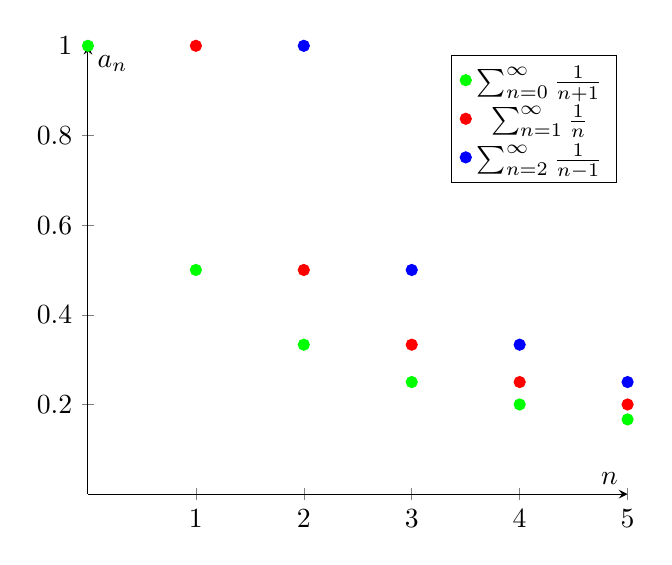
\begin{tikzpicture}
        \begin{axis}[axis lines = center, xmin = 0, xmax = 5, ymin = 0, 
        xlabel = $n$, ylabel = $a_n$]
        \addplot[green, mark=*, only marks] coordinates {
        (0, 1) (1, 1/2) (2, 1/3) (3, 1/4) (4, 1/5) (5, 1/6)};
        \addlegendentry{$\sum_{n=0}^\infty \frac{1}{n+1}$};
        \addplot[red, mark=*, only marks] coordinates {
        (1, 1) (2, 1/2) (3, 1/3) (4, 1/4) (5, 1/5)};
        \addlegendentry{$\sum_{n=1}^\infty \frac{1}{n}$};
        \addplot[blue, mark=*, only marks] coordinates {
        (2, 1) (3, 1/2) (4, 1/3) (5, 1/4)};
        \addlegendentry{$\sum_{n=2}^\infty \frac{1}{n-1}$};
        \end{axis}
\end{tikzpicture}
    \caption{$\sum_{n=0}^\infty \frac{1}{n + 1} = \sum_{n=1}^\infty a_n = 
    \sum_{n=2}^\infty = 1 + \frac{1}{2} + \frac{1}{3} + \cdots$}
    \label{fig:reindex}
\end{figure}

We can also prove each reindexing rule mathematically. Recall that 
$$\sum_{n=1}^\infty a_n = a_1 + a_2 + a_3 + \cdots$$
We also know that 
$$\sum_{n=2}^\infty a_{n-1} = a_{2-1} + a_{3-1} + a_{4-1} + \cdots = a_1 + a_2 
+ a_3 + \cdots$$
Therefore, $\sum_{n=1}^\infty a_n = \sum_{n=2}^\infty a_{n-1}$. 

Similarly, 
$$\sum_{n=0}^\infty a_{n + 1} = a_{0+1} + a_{1+1} + a_{2+1} + \cdots = a_1 + 
a_2 + a_3 + \cdots = \sum_{n=1}^\infty a_n$$

\textbf{Example}: Reindex the series $\sum_{n=3}^\infty \frac{n + 1}{n^2 - 2}$ 
to begin with $n=1$.

\textbf{Solution}: We are decreasing the index, so we will use $\sum_{n=i-1}^
\infty a_{n+1} = \sum_{n=i}^\infty a_n$. We will apply this rule twice, to 
decrease the index from 3 to 1:
$$\sum_{n=2}^\infty \frac{(n + 1) + 1}{(n + 1)^2 - 2} = \sum_{n=2}^\infty 
\frac{n + 2}{(n + 1)^2 - 2}$$
$$\sum_{n=1}^\infty \frac{(n + 1) + 2}{\left[ (n + 1) + 1 \right]^2 - 2} = 
\sum_{n=1}^\infty \frac{n + 3}{(n + 2)^2 - 2}$$

It is easier and faster to be able to reindex a series by more than one step 
at a time. Using the example above, we can write an even more general rule for 
reindexing:
$$\sum_{n=i}^\infty a_n = \sum_{n=i + j}^\infty a_{n - j}$$
where $i$ and $j$ are integers. (Then to decrease the index, you would choose 
a $j$ such that $j < 0$.)

\section{Convergent and Divergent Series}
Just like sequences, series can also be convergent or divergent. 
Consider the series $\sum_{i=1}^\infty i$. Given what you already 
know about the meaning of "convergent" and "divergent", guess whether 
$\sum_{i=1}^\infty i$ is convergent or divergent. 

Let's determine the first few partial sums of the series (shown 
graphically in figure \ref{fig:divsum}):
\begin{center}
\begin{tabular}{|c|c|c|}\hline
n & Terms & Partial Sum\\
\hline
1 & 1 & 1\\
\hline
2 & 1+2 & 3\\
\hline
3 & 1+2+3 & 6\\
\hline
4 & 1+2+3+4 & 10\\
\hline
\end{tabular}
\end{center}

\begin{figure}[htbp]
\centering
    \begin{tikzpicture}
        \begin{axis}[axis lines = center, xmin = -0.5, xmax = 10, 
        ymin = 0, ymax = 55, xlabel=n, ylabel = $s_n$]
        \addplot[blue, mark=*](1,1);
        \addplot[blue, mark=*](2, 3);
        \addplot[blue, mark=*](3, 6);
        \addplot[blue, mark=*](4, 10);
        \addplot[blue, mark=*](5, 15);
        \addplot[blue, mark=*](6, 21);
        \addplot[blue, mark=*](7, 28);
        \addplot[blue, mark=*](8, 36);
        \addplot[blue, mark=*](9, 45);
        \addplot[blue, mark=*](10,55);
        \end{axis}
\end{tikzpicture}
    \caption{For the divergent series $\sum_{i=1}^n i$, the value of the 
    partial sum increases to infinity as $n$ increases}
    \label{fig:divsum}
\end{figure}

As you can see, as $n$ increases, the value of the partial sum 
increases without approaching a particular value. We can also see 
that the value of the first $n$ terms summed together is 
$\frac{n(n+1)}{2}$. This means that as $n$ approaches $\infty$, the 
sum also approaches $\infty$ and the series is divergent. 

Obviously, for a series to not become huge, the values of the terms 
should decrease as $i$ increases (that is, each subsequent term is 
smaller than the one before it). Take the series $\sum_{i=1}^\infty 
\frac{1}{2^i}$. As $i$ increases, $\frac{1}{2^i}$ decreases. Let's 
look at the first few partial sums of this series (shown graphically 
in figure \ref{fig:convsum}):
\begin{center}
\begin{tabular}{|c|c|c|}\hline
n & Terms & Partial Sum\\
\hline
1 & $\frac{1}{2}$ & $\frac{1}{2}$\\
\hline
2 & $\frac{1}{2} + \frac{1}{4}$ & $\frac{3}{4}$\\
\hline
3 & $\frac{1}{2} + \frac{1}{4} + \frac{1}{8}$ & $\frac{7}{8}$\\
\hline
4 & $\frac{1}{2} + \frac{1}{4} + \frac{1}{8} + \frac{1}{16}$ & 
$\frac{15}{16}$\\
\hline
\end{tabular}
\end{center}

\begin{figure}[htbp]
\centering
    \begin{tikzpicture}
        \begin{axis}[axis lines = center, xmin = -0.5, xmax = 8, 
        ymin = 0, ymax = 1.5, ytick = {1}, xlabel=n, ylabel = $s_n$]
        \addplot[blue, mark=*](1,0.5);
        \addplot[blue, mark=*](2, 3/4);
        \addplot[blue, mark=*](3, 7/8);
        \addplot[blue, mark=*](4, 15/16);
        \addplot[blue, mark=*](5, 31/32);
        \addplot[blue, mark=*](6, 63/64);
        \addplot[blue, mark=*](7, 127/128);
        \addplot[blue, mark=*](8, 255/256);
        \addplot[red, thin, dashed, domain = 0:8]{1};
        \end{axis}
\end{tikzpicture}
    \caption{For the convergent series $\sum_{i=1}^n \frac{1}{2^i}$, 
    the value of the partial sum approaches 1 as $n$ increases}
    \label{fig:convsum}
\end{figure}

Do you see the pattern? The $n^{th}$ partial sum is equal to 
$\frac{2^n - 1}{2^n} = 1 - \frac{1}{2^n}$. And as $n$ approaches 
$\infty$, the partial sum approaches 1. The series $\sum_{i=1}^\infty 
\frac{1}{2^i}$ is convergent. 

Let us define the sequence \{$s_n$\} where $s_n$ is the $n^{th}$ 
partial sum of a series:
$$s_n = \sum_{i=1}^n a_i$$. 

If the sequence \{$s_n$\} is convergent and $\lim_{n \to \infty} s_n$ 
exists, then the series $\sum_{i=1}^\infty a_i$ is also convergent. 
And if the sequence \{$s_n$\} is divergent, then the series 
$\sum_{i=1}^\infty a_i$ is also divergent.

\textbf{Example}: is the harmonic series, $\sum_{n = 1}^\infty \frac{1}{n}$ 
convergent or divergent?

\textbf{Solution}: You may think that the series is convergent, since $\lim_
{n \to \infty} \frac{1}{n} = 0$. Let's see if we can confirm this. We begin by 
looking at the partial sums $s_2$, $s_4$, $s_8$, and $s_{16}$:
$$s_2 = 1 + \frac{1}{2}$$
$$s_4 = 1 + \frac{1}{2} + \left(\frac{1}{3} + \frac{1}{4} \right) > 1 + 
\frac{1}{2} + \left( \frac{1}{4} + \frac{1}{4} \right) = 1 + \frac{2}{2}$$
$$s_8 = 1 + \frac{1}{2} + \left(\frac{1}{3} + \frac{1}{4} \right) + \left( 
\frac{1}{5} + \frac{1}{6} + \frac{1}{7} + \frac{1}{8} \right) > 1 + \frac{1}{2} 
+ \left(\frac{1}{4} + \frac{1}{4} \right) + \left( \frac{1}{8} + \frac{1}{8} + 
\frac{1}{8} + \frac{1}{8} \right) = 1 + \frac{3}{2}$$
$$s_{16} = 1 + \frac{1}{2} + \left(\frac{1}{3} + \frac{1}{4} \right) + \left( 
\frac{1}{5} + \frac{1}{6} + \frac{1}{7} + \frac{1}{8} \right) + \left(
\frac{1}{9} + \cdots + \frac{1}{16} \right) > $$
$$1 + \frac{1}{2} + \left(\frac{1}{4} + \frac{1}{4} \right) + \left( 
\frac{1}{8} + \frac{1}{8} + \frac{1}{8} + \frac{1}{8} \right) + \left(
\frac{1}{16} + \cdots + \frac{1}{16} \right) = 1 + \frac{4}{2}$$

Notice that, in general, $s_{2^n} > 1 + \frac{n}{2}$ for $n > 1$. Taking the 
limit as $n \to \infty$, we see that $\lim_{n \to \infty} s_{2^n} > \lim_{n 
\to \infty} 1 + \frac{n}{2} = \infty$. Therefore, $s_{2^n}$ also approaches 
$\infty$ as $n$ gets larger and the harmonic series $\sum_{n = 1}^\infty 
\frac{1}{n}$ is divergent. 

This example shows a very important point: a series whose terms decrease to 
zero as n gets large is not necessarily convergent. What we can say, though, 
is that if the limit as n approaches infinity of the terms of a series does not 
exist or is not zero, then the series is divergent (i.e. not convergent). This 
is called the \textbf{Test for Divergence}, and we will explore it further in 
the next chapter. \index{Test for Divergence}

\subsection{Properties of Convergent Series}
We just saw that if $\lim_{n \to \infty} a_n \neq 0$ then the series $\sum_
{n=1}^\infty a_n$ diverges. The contrapositive statement gives a property of 
convergent series:
$$\text{If the series } \sum_{n=1}^\infty a_n \text{ is convergent, then } 
\lim_{n \to \infty} = 0$$

If a series is made of other convergent series, it may be convergent. Recall, 
if a series is convergent, this means the $\lim_{n \to \infty} \sum_{i=1}^n 
a_i = L$. By the properties of limits, then we can also say that the series 
multiplied by a constant is convergent:
$$\sum_{n=1}^\infty ca_n = c \cdot L = c \sum_{n=1}^\infty a_n$$
Suppose there is another convergent series such that $\lim_{n \to \infty} 
\sum_{i=1}^n b_i = M$. Then the sum of those series is also convergent. That is:
$$\sum_{n=1}^\infty \left( a_n + b_n \right) = L + M = \sum_{n=1}^\infty a_n + 
\sum_{n=1}^\infty b_n$$
Similarly, the difference of the series is convergent:
$$\sum_{n=1}^\infty \left( a_n - b_n \right) = L - M = \sum_{n=1}^\infty a_n - 
\sum_{n=1}^\infty b_n$$

\section{Geometric Series}

A geometric series is the sum of a geometric sequence, and has the form:
$$\sum_{n=1}^\infty ar^n \text{ or } \sum_{n=1}^\infty ar^{n-1}$$ \index{geometric series}

Where $a$ is some constant and $r$ is the common ratio. For $\sum_{n=1}^\infty 
ar^{n-1}$, $a$ is also the first term. 

\textbf{Example}: Write the series $1 + \frac{1}{2} + \frac{1}{4} + 
\frac{1}{8} + \cdots$ in sigma notation.

\textbf{Solution}: We see that the first term is $a=1$ and the common ratio is 
$\frac{1}{2}$, so we can write the series: $$\sum_{n=1}^\infty 1(\frac{1}{2})^
{n-1} = \sum_{n=1}^\infty (\frac{1}{2})^{n-1}$$

When are geometric series convergent? First, let's consider the case 
where $r=1$. If this is true, then $s_n = a + a + a + \cdots + a = 
na$. As $n$ approaches $\infty$, the sum will approach $\pm \infty$ 
(depending on whether $a$ is positive or negative), and the series is 
divergent. 

When $r \neq 1$, we can write $s_n$ and $rs_n$:
$$s_n = a + ar + ar^2 + \cdots + ar^{n-1}$$
$$rs_n = ar + ar^2 + ar^3 + \cdots + ar^n$$

Subtracting $rs_n$ from $s_n$, we get:
$$s_n - rs_n = (a + ar + ar^2 + \cdots + ar^{n-1}) - (ar + ar^2 + 
ar^3 + \cdots + ar^{n-1} + ar^n)$$
$$= a - ar^n$$

Solving for $s_n$, we find:
$$s_n = \frac{a(1-r^n)}{1-r}$$

We take the limit as $n \to \infty$ to determine for what values of 
$r$ the series converges:
$$\lim_{n \to \infty} s_n = \lim_{n \to \infty} \frac{a(1-r^n)}{1-r}$$
$$= \lim_{n\to \infty} \left[ \frac{a}{1-r} - \frac{ar^n}{1-r} \right] = \frac{a}{1-r} 
- \left( \frac{a}{1-r} \right) \lim_{n \to \infty} r^n$$

This begs the question: when is $\lim_{n \to \infty} r^n$ convergent? 
From the sequences chapter, we know this limit converges if $|r| < 1$ 
(that is, $-1 < r < 1$). If this is true, then $\lim_{n \to \infty} 
r^n = 0$ and 
$$\lim_{n \to \infty} s_n = \frac{a}{1-r}$$

(see figures \ref{fig:geometric1} and \ref{fig:geometric2} for a visual)
\begin{figure}
    \centering
    \begin{tikzpicture}
        \begin{axis}[xmin = -0.5, xmax = 10, ymin = 0, axis lines = center, 
        xlabel = $n$, clip = false, ytick = \empty]
        \addplot[red, mark=*] (1, 2); %r=1.5
        \addplot[red, mark=*] (2, 5);
        \addplot[red, mark=*] (3, 19/2);
        \addplot[red, mark=*] (4, 65/4);
        \addplot[red, mark=*] (5, 211/8);
        \addplot[red, mark=*] (6, 665/16);
        \addplot[red, mark=*] (7, 2059/32);
        \node[red] at (5.5, 60) {$r > 1$};
        
        \addplot[orange, mark=*] (1, 2); %r=1
        \addplot[orange, mark=*] (2, 4);
        \addplot[orange, mark=*] (3, 6);
        \addplot[orange, mark=*] (4, 8);
        \addplot[orange, mark=*] (5, 10);
        \addplot[orange, mark=*] (6, 12);
        \addplot[orange, mark=*] (7, 14);
        \addplot[orange, mark=*] (8, 16);
        \addplot[orange, mark=*] (9, 18);
        \addplot[orange, mark=*] (10, 20);
        \node[orange] at (9, 25) {$r = 1$};
        
        \addplot[blue, mark =*] (1, 2); %r = 0.5
        \addplot[blue, mark =*] (2, 3);
        \addplot[blue, mark =*] (3, 7/2);
        \addplot[blue, mark =*] (4, 15/4);
        \addplot[blue, mark =*] (5, 31/8);  
        \addplot[blue, mark =*] (6, 63/16);
        \addplot[blue, mark =*] (7, 127/32);
        \addplot[blue, mark =*] (8, 255/64);
        \addplot[blue, mark =*] (9, 511/128);
        \addplot[blue, mark =*] (10, 1023/256);
        \node[blue] at (10, 10) {$0 < r < 1$};
        \end{axis}
    \end{tikzpicture}
    \caption{Geometric sequences are divergent if $r \geq 1$}
    \label{fig:geometric1}
\end{figure}

\begin{figure}
    \centering
    \begin{tikzpicture}
        \begin{axis}[xmin = -0.5, xmax = 10, axis lines = center, 
        xlabel = $n$, clip = false, ytick = \empty]
        \addplot[red, mark=*] (1, 2); %r=-1.5
        \addplot[red, mark=*] (2, -1);
        \addplot[red, mark=*] (3, 7/2);
        \addplot[red, mark=*] (4, -13/4);
        \addplot[red, mark=*] (5, 55/8);
        \addplot[red, mark=*] (6, -133/16);
        \addplot[red, mark=*] (7, 463/32);
        %\addplot[red, mark=*] (8, -1261/64);
        %\addplot[red, mark=*] (9, 4039/128);
        %\addplot[red, mark=*] (10, -11605/256);
        \node[red] at (5, 10) {$r > 1$};
        
        \addplot[orange, mark=*] (1, 2); %r=-1
        \addplot[orange, mark=*] (2, 0);
        \addplot[orange, mark=*] (3, 2);
        \addplot[orange, mark=*] (4, 0);
        \addplot[orange, mark=*] (5, 2);
        \addplot[orange, mark=*] (6, 0);
        \addplot[orange, mark=*] (7, 2);
        \addplot[orange, mark=*] (8, 0);
        \addplot[orange, mark=*] (9, 2);
        \addplot[orange, mark=*] (10, 0);
        \node[orange] at (9, -3) {$r = -1$};
        
        \addplot[blue, mark =*] (1, 2); %r = -0.5
        \addplot[blue, mark =*] (2, 1);
        \addplot[blue, mark =*] (3, 3/2);
        \addplot[blue, mark =*] (4, 5/4);
        \addplot[blue, mark =*] (5, 11/8);  
        \addplot[blue, mark =*] (6, 21/16);
        \addplot[blue, mark =*] (7, 43/32);
        \addplot[blue, mark =*] (8, 85/64);
        \addplot[blue, mark =*] (9, 171/128);
        \addplot[blue, mark =*] (10, 341/256);
        \node[blue] at (9, 5) {$-1 < r < 0$};
        \end{axis}
    \end{tikzpicture}
    \caption{Geometric sequences are divergent if $r \leq 1$. Notice that for 
    $r = -1$, the partial sums alternate between the initial term and zero.}
    \label{fig:geometric2}
\end{figure}

\textbf{Example}: Find the sum of the geometric series given by $2 - 
\frac{2}{3} + \frac{2}{9} - \frac{2}{27} + \cdots$. 

\textbf{Solution}: The first term is $a = 2$ and each the common 
ratio is $r = \frac{-1}{3}$. Since $|r| < 1$, we know that the series 
converges. We can calculate the value of the sum using the geometric 
series formula: 
$$\sum_{i=1}^\infty a(r)^{i-1} = \frac{a}{1-r}$$
$$\sum_{i=1}^\infty 2(\frac{-1}{3})^{i-1} = \frac{2}{1-\frac{-1}{3}} = 
\frac{2}{\frac{4}{3}} = \frac{6}{4} = 1.5$$

We can confirm this graphically (see figure \ref{fig:geometric}). You 
can also write out the first several partial sequences: you should 
find the sums approach 1.5 as $n$ increases.

\begin{figure}[htbp]
\centering
    \begin{tikzpicture}
        \begin{axis}[axis lines = center, xmin = -0.5, xmax = 8, 
        ymin = -1.5, ymax = 2, xlabel=n, legend pos = south east]
        \addplot[blue, mark=*](1,2);
        \addlegendentry{$s_n$};
        \addplot[red, mark=o](1, 2);
        \addlegendentry{$a_n$};
        \addplot[blue, mark=*](2, 4/3);
        \addplot[blue, mark=*](3, 14/9);
        \addplot[blue, mark=*](4, 40/27);
        \addplot[blue, mark=*](5, 122/81);
        \addplot[blue, mark=*](6, 364/243);
        \addplot[blue, mark=*](7, 1094/729);
        \addplot[blue, mark=*](8, 3280/ 2187);
        \addplot[red, mark=o](2, -2/3);
        \addplot[red, mark=o](3, 2/9);
        \addplot[red, mark=o](4, -2/27);
        \addplot[red, mark=o](5, 2/81);
        \addplot[red, mark=o](6, -2/243);
        \addplot[red, mark=o](7, 2/729);
        \addplot[red, mark=o](8, -2/2187);
        \addplot[red, thin, dashed, domain = 0:8]{1.5};
        \end{axis}
\end{tikzpicture}
    \caption{the $n^{th}$ term and partial sums of $\sum_{i=1}^n 
    2(\frac{-1}{3})^{i-1}$}
    \label{fig:geometric}
\end{figure}

\textbf{Example}: What is the value of $\sum_{n=1}^\infty 2^{2n}5^{1-n}$

\textbf{Solution}: The key here is to re-write the series in the form $\sum_
{n=1}^\infty ar^{n -1}$ so we can use the fact that convergent geometric 
series sum to $\frac{a}{1-r}$. 
$$\sum_{n=1}^\infty 2^{2n}5^{1-n} = \sum_{n=1}^\infty \left( 2^2 \right)^n 
\left( \frac{1}{5} \right)^{n-1}$$
$$= \sum_{n=1}^\infty 4 \cdot \left( 4 \right)^{n-1} \left( \frac{1}{5} 
\right)^{n-1} = \sum_{n=1}^\infty 4 \cdot \left( \frac{4}{5} \right)^{n-1}$$
Which is in the form $\sum_{n=1}^\infty ar^{n -1}$ with $a=4$ and $r=
\frac{4}{5}$. Since $|r| < 1$, the series converges to 
$$\frac{a}{1-r} = \frac{4}{1-\frac{4}{5}} = \frac{4}{\frac{1}{5}} = 20$$

\begin{Exercise}[label=geo1]
Determine whether the geometric series is convergent or divergent. If it 
convergent, find its sum.
\begin{enumerate}
\item $3 - 4 + \frac{16}{3} - \frac{64}{9} + \cdots$
\item $2 + 0.5 + 0.125 + 0.03125 + \cdots$
\item $\sum_{n=1}^\infty \frac{(-3)^{n-1}}{4^n}$
\item $\sum_{n=1}^\infty \frac{e^{2n}}{6^{n-1}}$
\end{enumerate}
\end{Exercise}

\begin{Answer}[ref = geo1]
\begin{enumerate}
\item We need to identify $a$ and $r$. If we use the form $\sum_{n=1}^\infty 
ar^{n-1}$, then $a = 3$. To find the common ratio, we can evaluate $\frac{a_
{n+1}}{a_n} = \frac{-4}{3}$. Then we can write the series as $\sum_{n=1}^\infty 
3 \left( \frac{-4}{3} \right)^{n-1}$. In this case, $r = \frac{-4}{3}$ and $|r| 
\geq 1$, and therefore the series is divergent. 
\item Following the process outlined above, we see that $a = 2$ and $r = 
\frac{1}{4}$. Therefore the series is $\sum_{n=1}^\infty 2 \left( \frac{1}{4} 
\right)^{n-1}$. Since $|r| < 1$, the series converges to $\frac{a}{1-r} = 
\frac{2}{1-1/4} = \frac{2 \cdot 4}{3} = \frac{8}{3}$
\item We need to rewrite the series into a standard from in order to identify 
$a$ and $r$:
$$\sum_{n=1}^\infty \frac{(-3)^{n-1}}{4^n} = \sum_{n=1}^\infty \frac{(-3)^
{n-1}}{4(4)^{n-1}} = \sum_{n=1}^\infty \frac{1}{4} \left( \frac{-3}{4} \right)
^{n-1}$$
So $r = \frac{-3}{4}$ and $|r| < 1$. Therefore, the series converges to 
$\frac{1/4}{1 - (-3/4)} = \frac{1}{4} \cdot \frac{4}{7} = \frac{1}{7}$
\item We need to rewrite the series into a standard from in order to identify 
$a$ and $r$:
$$\sum_{n=1}^\infty \frac{e^{2n}}{6^{n-1}} = \sum_{n=1}^\infty \frac{(e^2)^n}
{6^{n-1}} = \sum_{n=1}^\infty \frac{(e^2)(e^2)^{n-1}}{6^{n-1}} = \sum_{n=1}^
\infty e^2 \left( \frac{e^2}{6} \right)^{n-1}$$
Therefore, $r = \frac{e^2}{6} \approx 1.232$. Since $|r| > 1$, the series 
diverges. 
\end{enumerate}
\end{Answer}

\begin{Exercise}[label = geo2]
Find a value of $c$ such that $\sum_{n=0}^\infty (1 + c)^{-n} = \frac{5}{3}$
\end{Exercise}

\begin{Answer}[ref = geo2]
We want to rewrite this as a geometric series of the form $\sum_{n=i}^\infty 
ar^{n-1}$ so we can use the fact that the sum of a convergent geometric series 
is $\frac{a}{1-r}$. $\sum_{n=0}^\infty (1 + c)^{-n} = \sum_{n=0}^\infty \left( 
\frac{1}{1+c} \right)^n = \sum_{n=1}^\infty \left( \frac{1}{1 + c} \right)^
{n-1}$. This is a geometric series with $a = 1$ and $r = \frac{1}{1 + c}$. So 
the value of the series is $\frac{1}{1 - \frac{1}{1+c}} = 
\frac{1}{\frac{c}{c+1}} = \frac{c+1}{c}$. Setting this equal to $\frac{5}{3}$ 
and solving for $c$, we find that $c = \frac{3}{2}$.
\end{Answer}

\begin{Exercise}[label = geo3]
For what values of $p$ does the series $\sum_{n = 1}^\infty \left( \frac{p}{2} 
\right) ^ n$ converge?
\end{Exercise}

\begin{Answer}[ref = geo3]
$-2 < p < 2$ Let's re-write this geometric series into standard form: $\sum_{n 
= 1}^\infty \left( \frac{p}{2} \right) ^ n = \sum_{n = 1}^\infty \frac{p}{2} 
\left( \frac{p}{2} \right) ^ n$ which means $a = \frac{p}{2}$ and $r = 
\frac{p}{2}$. We know that geometric series converge if $\left| r \right| < 
1$, so we set up an inequality and solve for $p$:
$$\left| \frac{p}{2} \right| < 1$$
$$-1 < \frac{p}{2} < 1$$
$$-2 < p < 2$$
\end{Answer}

\section{p-series}
A $p$-series takes the form $\sum_{n=1}^\infty \frac{1}{n^p}$ and converges 
if $p > 1$ and diverges if $p \leq 1$. We won't prove this here, since it 
requires the application of a test you will learn about in the next chapter. \index{p-series}

\textbf{Example} Write the series $1 + \frac{1}{\sqrt[3]{2}} + \frac{1}{
\sqrt[3]{3}} + \frac{1}{\sqrt[3]{4}} + \cdots$. Is it convergent or divergent?

\textbf{Solution}: We see that $a_n = \frac{1}{\sqrt[3]{n}}$ and so the 
infinite series is $$\sum_{n=1}^\infty \frac{1}{\sqrt[3]{n}}$$ 
We see that this is a $p$-series with $p = \frac{1}{3}$. Since $p < 1$, the 
series is divergent. 

\begin{Exercise}[label = euler1]
Euler found that the exact sum of the p-series where $p=2$ is:
$$\sum_{n=1}^\infty \frac{1}{n^2} = \frac{\pi^2}{6}$$
And that the exact sum of the p-series where $p=4$ is:
$$\sum_{n=1}^\infty \frac{1}{n^4} = \frac{\pi^4}{90}$$
Use this and the properties of convergent series to find the sum of each of 
the following series:
\begin{enumerate}
\item $\sum_{n=1}^\infty \frac{n^2 + 1}{n^4}$
\item $\sum_{n=2}^\infty \frac{1}{n^2}$
\item $\sum_{n=3}^\infty \frac{1}{(n + 1)^2}$
\item $\sum_{n=1}^\infty \left( \frac{3}{n} \right)^4$
\item $\sum_{n=1}^\infty \left( \frac{4}{n^2} + \frac{3}{n^4} \right)$
\end{enumerate}
\vspace{50mm}
\end{Exercise}

\begin{Answer}[ref = euler1]
\begin{enumerate}
\item Separating the terms, we see that $\sum_{n=1}^\infty \frac{n^2 + 1}{n^4} 
= \sum_{n=1}^\infty \left( \frac{n^2}{n^4} + \frac{1}{n^4} \right) = \sum_{n=1}
^\infty \frac{1}{n^2} + \sum_{n=1}^\infty \frac{1}{n^4} = \frac{\pi^2}{6} + 
\frac{\pi^4}{90}$
\item Notice that this series starts at $n = 2$. By the properties of series, 
we know that $\sum_{n=1}^\infty a_n = a_1 + \sum_{n=2}^\infty a_n$. Therefore, 
$\sum_{n=2}^\infty \frac{1}{n^2} = \sum_{n=1}^\infty \left( \frac{1}{n^2} 
\right) - \frac{1}{1^2} = \frac{\pi^2}{6} - 1$
\item We can begin by reindexing this series: $\sum_{n=3}^\infty \frac{1}{(n + 
1)^2} = \sum_{n=4}^\infty \frac{1}{n^2}$. Similar to the previous problem, we 
also know that $\sum_{n=4}^\infty \frac{1}{n^2} = \sum_{n=1}^\infty \left( 
\frac{1}{n^2} \right) - \left( \frac{1}{1^2} + \frac{1}{2^2} + \frac{1}{3^2} 
\right) = \frac{\pi^2}{6} - \frac{49}{36}$
\item We can re-write this series as $\sum_{n=1}^\infty \left( \frac{3}{n} 
\right)^4 = \sum_{n=1}^\infty (3^4)\frac{1}{n^4} = 81 \sum_{n=1}^\infty 
\frac{1}{n^4} = \frac{81\pi^4}{90} = \frac{9\pi^4}{10}$
\item We can re-write the series as $\sum_{n=1}^\infty \left( \frac{4}{n^2} + 
\frac{3}{n^4} \right) = \sum_{n=1}^\infty \frac{4}{n^2} + \sum_{n=1}^\infty 
\frac{3}{n^4} = 4 \sum_{n=1}^\infty \frac{1}{n^2} + 3 \sum_{n=1}^\infty 
\frac{1}{n^4} = \frac{4\pi^2}{6} + \frac{3\pi^4}{90} = \frac{2\pi^2}{3} + 
\frac{\pi^4}{30}$
\end{enumerate}
\end{Answer}

\begin{Exercise}[label = pseries1]
For what values of $k$ does the series $\sum_{n = 1}^\infty \frac{1}{n^{2k}}$ 
converge?
\end{Exercise}

\begin{Answer}[ref = pseries1]
This is a $p$-series where $p = 2k$. We know that $p$-series converge for $p > 
1$: $2k > 1 \rightarrow k > \frac{1}{2}$. 
\end{Answer}

\section{Alternating Series}
An alternating series is one in which the terms alternate between positive and 
negative \index{alternating series}. Here is an example:
$$-\frac{1}{2} + \frac{2}{3} - \frac{3}{4} + \frac{4}{5} - \frac{5}{6} + 
\cdots = \sum_{n=1}^\infty (-1)^n \frac{n}{n + 1}$$
Alternating series are generally of the form
$$a_n = (-1)^n b_n \text{ or } a_n = (-1)^{n - 1} b_n$$
Where $b_n$ is positive (and therefore, $|a_n| = b_n$).

An alternating series is convergent if (i)$b_{n+1} \leq b_n$ and (ii)$\lim_{n 
\to \infty} b_n = 0$. In words, we say that if the absolute value of the terms 
of a series decrease towards zero, then the series converges. This is called 
the \textbf{Alternating Series Test}. \index{Alternating Series Test}

\begin{figure}[htbp]
\centering
    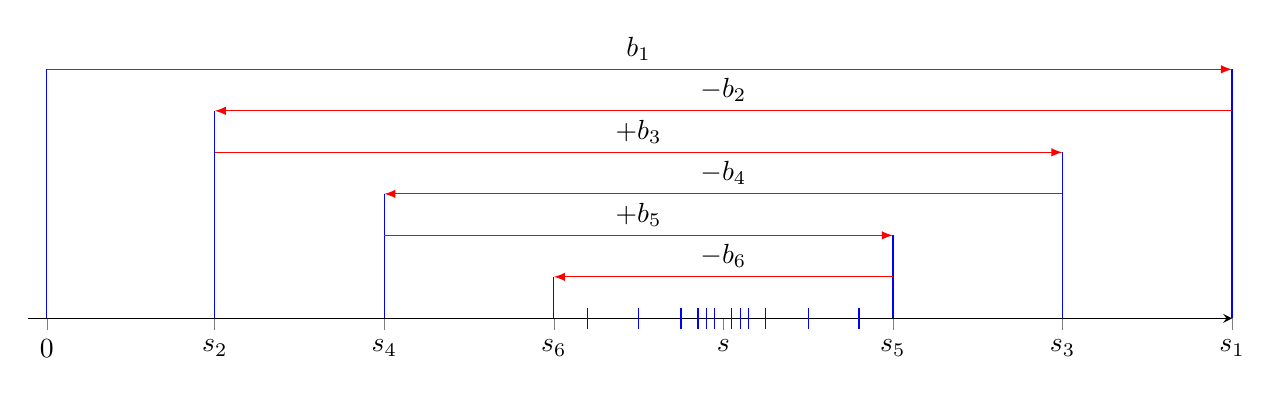
\begin{tikzpicture}
        \begin{axis}[axis y line = none, width = 2*\axisdefaultwidth, 
        height = 0.25*\axisdefaultwidth, axis lines = center, 
        xtick align = outside, xmin = -0.1, xmax = 7, 
        xtick = {0.01, 1, 2, 3, 4, 5, 6, 7}, xticklabels = {$0$, $s_2$, $s_4$, 
        $s_6$, $s$, $s_5$, $s_3$, $s_1$}, ymin = -0.5, ymax = 0.5, 
        clip = false]
        \draw[blue](0.01, 0) -- (0.01, 6);
        \draw[blue](7, 0) -- (7, 6);
        \draw[red, -latex](0.01, 6) --(7, 6);
        \node[] at (3.5, 6.5) {$b_1$};
        \draw[blue] (1, 0) -- (1, 5);
        \draw[red, -latex] (7, 5) -- (1, 5);
        \node[] at (4, 5.5) {$- b_2$};
        \draw[blue] (6, 0) -- (6, 4);
        \draw[red, -latex] (1, 4) -- (6, 4);
        \node[] at (3.5, 4.5) {$+b_3$};
        \draw[blue] (2, 0) -- (2, 3);
        \draw[red, -latex] (6, 3) -- (2, 3);
        \node[] at (4, 3.5) {$-b_4$};
        \draw[blue] (5, 0) -- (5, 2);
        \draw[red, -latex] (2, 2) -- (5, 2);
        \node[] at (3.5, 2.5) {$+ b_5$};
        \draw[blue] (3, 0) -- (3, 1);
        \draw[red, -latex] (5, 1) -- (3, 1);
        \node[] at (4, 1.5) {$- b_6$};
        \draw[blue] (3.2, -0.25) -- (3.2, 0.25);
        \draw[blue] (4.8, -0.25) -- (4.8, 0.25);
        \draw[blue] (3.5, -0.25) -- (3.5, 0.25);
        \draw[blue] (4.5, -0.25) -- (4.5, 0.25);
        \draw[blue] (3.75, -0.25) -- (3.75, 0.25);
        \draw[blue] (4.25, -0.25) -- (4.25, 0.25);
        \draw[blue] (3.85, -0.25) -- (3.85, 0.25);
        \draw[blue] (4.15, -0.25) -- (4.15, 0.25);
        \draw[blue] (3.9, -0.25) -- (3.9, 0.25);
        \draw[blue] (4.1, -0.25) -- (4.1, 0.25);
        \draw[blue] (3.95, -0.25) -- (3.95, 0.25);
        \draw[blue] (4.05, -0.25) -- (4.05, 0.25);
        \end{axis}
\end{tikzpicture}
    \caption{As $n$ increases, $s_n$ approaches $s$}
    \label{fig:alternating}
\end{figure}

\textbf{Example}: Is the alternating harmonic series $\sum_{n=1}^\infty 
\frac{(-1)^{n-1}}{n}$ convergent?

\textbf{Solution}: The Alternating series test states that an alternating 
series is convergent if $|a_{n+1}| < |a_n|$:
$$\left| \frac{(-1)^{n-1+1}}{n+1} \right| < \left| \frac{(-1)^{n-1}}{n} \right|$$
$$\frac{1}{n+1} < \frac{1}{n}$$
Since $|a_{n+1}| < |a_n|$ and the series is alternating, $\sum_{n=1}^\infty 
\frac{(-1)^{n-1}}{n}$ is convergent. 

\begin{Exercise}[label=alt1]
Test the following alternating series for convergence:
\begin{enumerate}
\item $\sum_{n=1}^\infty \frac{(-1)^n 3n}{4n-1}$
\item $\sum_{n=1}^\infty (-1)^{n+1} \frac{n^2}{n^3 + 1}$
\item $\sum_{n=1}^\infty (-1)^{n-1} e^{2/n}$
\end{enumerate}
\vspace{50mm}
\end{Exercise}

\begin{Answer}[ref = alt1]
\begin{enumerate}
\item The series is convergent if $\left| \frac{(-1)^{n+1} 3(n+1)}{4(n+1)-1} 
\right| < \left| \frac{(-1)^n 3n}{4n-1} \right|$ if $\frac{3n+3}{4n+4-1} < 
\frac{3n}{4n-1}$ and if $\frac{3n+3}{4n+3} < \frac{3n}{4n-1}$ if $(3n+3)(4n-1) 
< (3n)(4n+3)$ if $12n^2 + 12n - 3n - 3 < 12n^2 + 9n$ if $-3 < 0$ which is true. 
Therefore, $\sum_{n=1}^\infty \frac{(-1)^n 3n}{4n-1}$ is convergent. 
\item The series is convergent if $\left| (-1)^{n+1+1} \frac{(n+1)^2}{(n+1)^3 
+ 1} \right| < \left| (-1)^{n+1} \frac{n^2}{n^3 + 1} \right|$ which is true if 
$\frac{(n+1)^2}{(n+1)^3 + 1} < \frac{n^2}{n^3 + 1}$ if $(n+1)^2 (n^3 + 1) < 
(n^2) ((n+1)^3+1)$ if $(n^2 + 2n + 1)(n^3) < (n^2) (n^3 + 3n^2 + 3n + 1 + 1)$ 
if $n^5 + 2n^4 + n^3 < n^5 + 3n^4 + 3n^3 + 2n^2$ which is true for all $n \geq 
1$. Therefore, $\sum_{n=1}^\infty (-1)^{n+1} \frac{n^2}{n^3 + 1}$ is convergent.
\item The series is convergent if $\left| (-1)^{n-1+1} e^{2/(n+1)} \right| < 
\left| (-1)^{n - 1} e^{2/n} \right|$ which is true if $e^{2/(n+1)} < e^{2/n}$ 
which is true if $\frac{2}{n+1} < \frac{2}{n}$ which is true for all $n \geq 1$. 
Therefore, $\sum_{n=1}^\infty (-1)^{n-1} e^{2/n}$ is convergent. 
\end{enumerate}
\end{Answer}






